%
%
%

\begin{frame}[t,allowframebreaks]{LeNet-5 -}

    \vspace{-0.2cm}
    \index{LeNet-5}\gls{LeNet-5} \cite{LeCun:1998ln5} 
    was the earliest convolutional network.\\
    \vspace{0.1cm}
    The network was {\bf quite shallow}: 
    It contained 2 convolution layers and 
    2 \index{pooling}\gls{pooling} layers, 
    followed by 3 fully connected layers.\\
    \begin{center}
        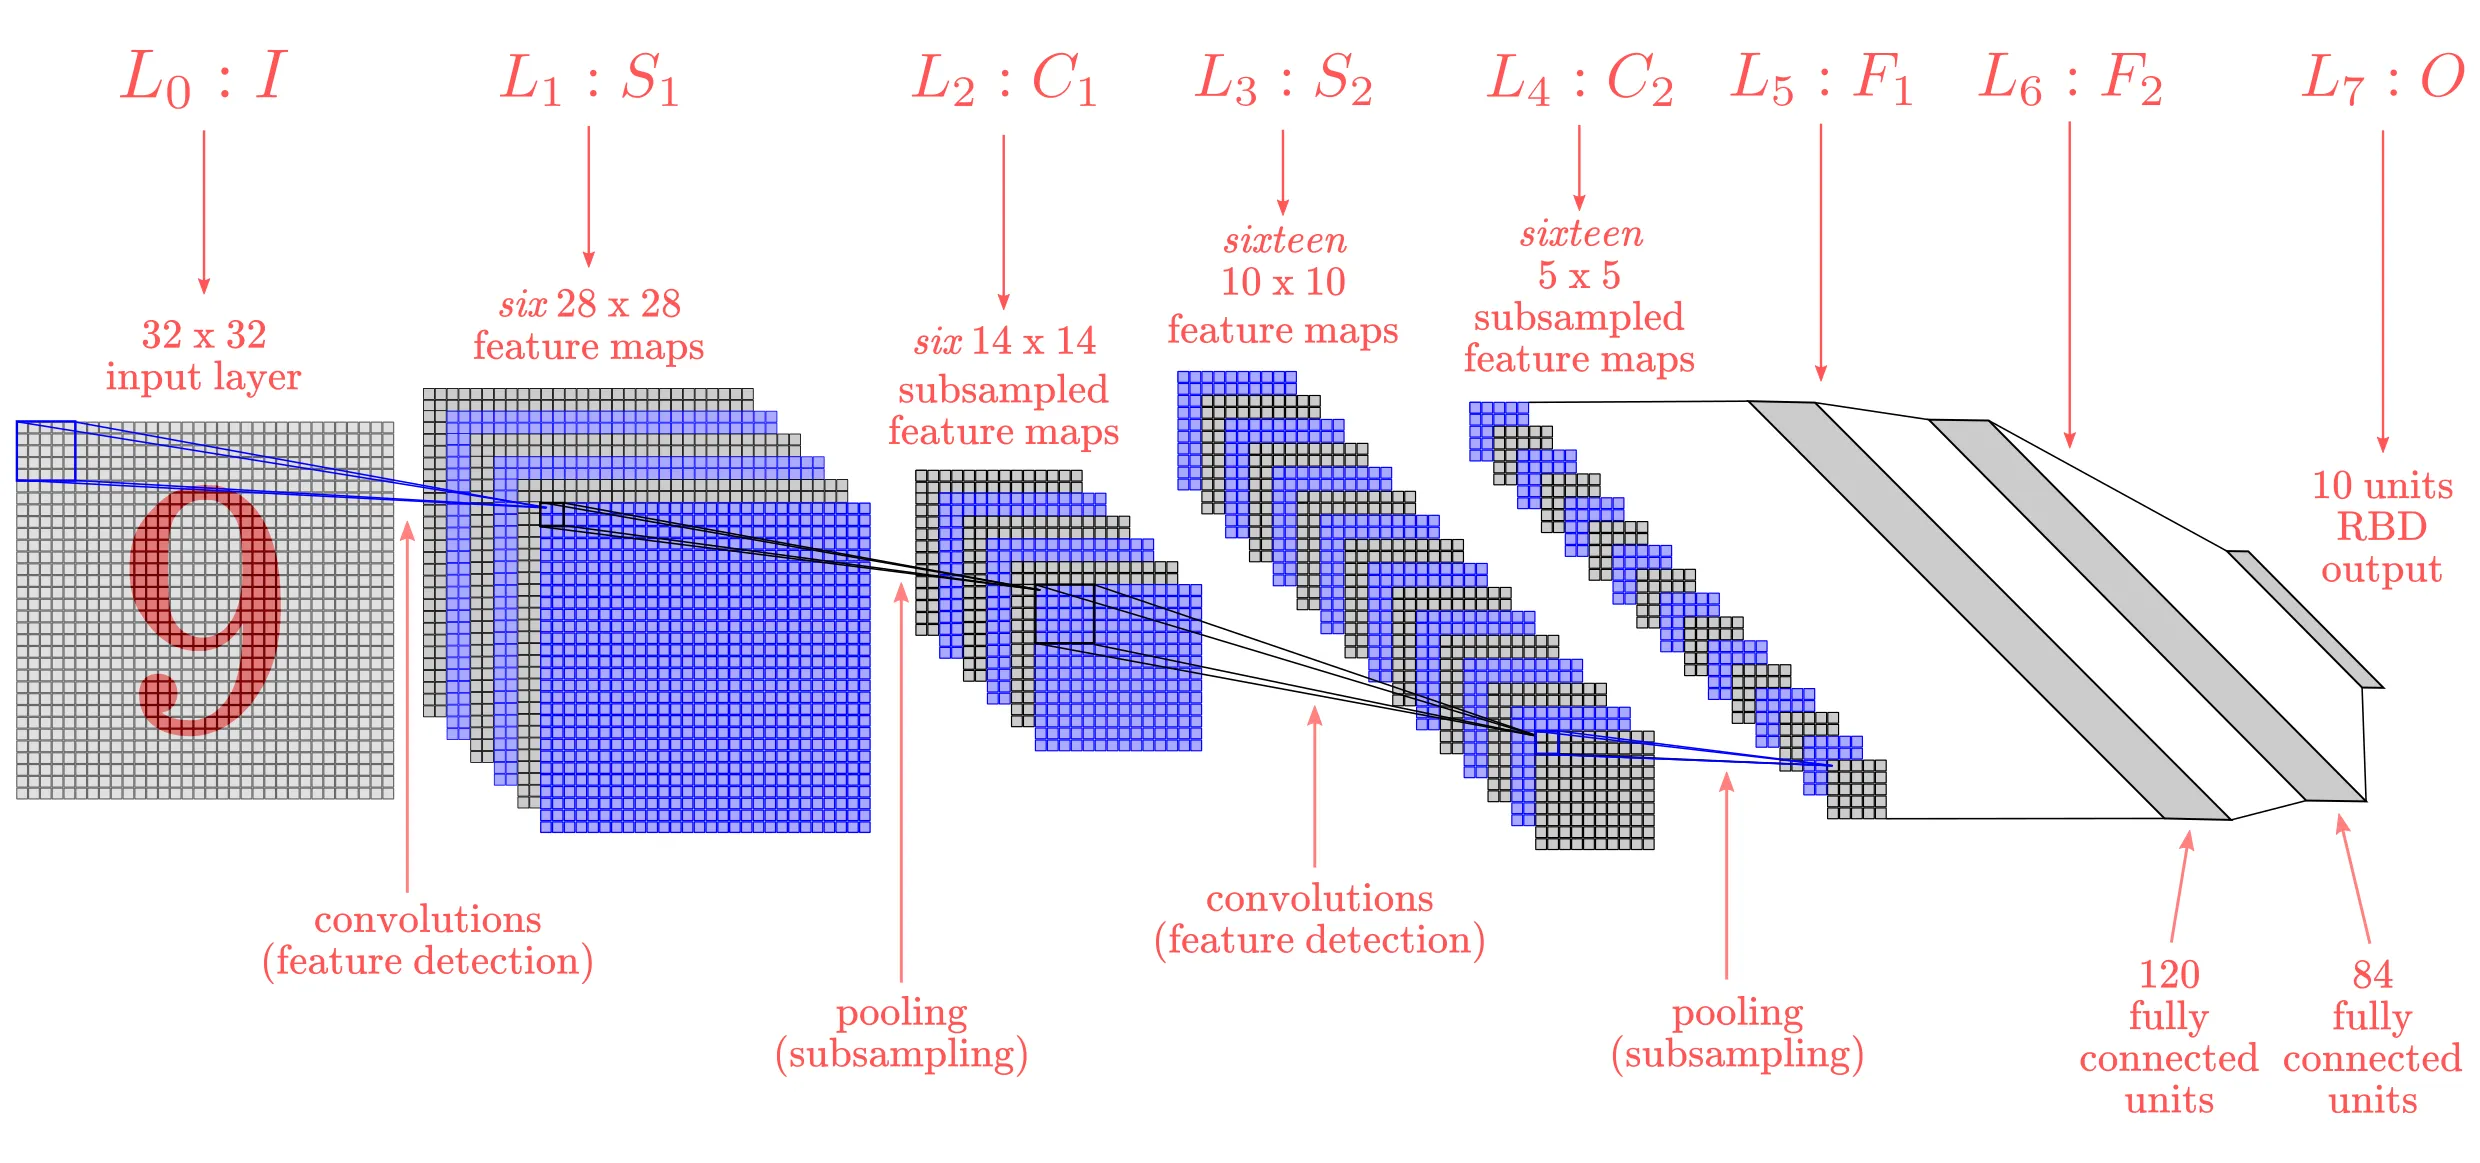
\includegraphics[width=0.97\textwidth]
            {./images/cnn/lenet5/elhamraoui20_lenet_architecture.png}\\
        \vspace{-0.5cm}
        {\scriptsize
            LeNet-5 architecture.
            \color{col:attribution} 
            Image reproduced from \cite{Medium:LeNet5andAlexNet}}\\    
    \end{center}

\end{frame}
